%!TEX root = ../main.tex

\section{Energy shift \& electron rest mass}
\label{sec:energy-shift}

In an attempt to estimate the rest mass of the electron, \autoref{eq:photon-energy}
can be rewritten.

\begin{equation}
\label{eq:linear-regression}
\frac{1}{E_{\gamma,f}} = \frac{1}{E_{\gamma,i}} + \frac{1}{m_e}\cdot\left(1-\cos\theta\right).
\end{equation}

According to \autoref{eq:linear-regression} the plot of $\frac{1}{E_{\gamma,f}}$ over
$(1-\cos\theta)$ should be a line with slope $\frac{1}{m_e}$ and intercept 
$\frac{1}{E_{\gamma,i}}$. A linear regression should be able to estimate $m_e$ from
the measurement data gathered in \autoref{sec:differential-cross-section}.

The photon energy $E_{\gamma,f}$ post-scattering can be directly extracted from the 
location of the gaussian peaks present in the measured compton spectra. 
A normal distribution is fitted to each peak. The results
of these processes are listed in \autoref{tab:energy-shift}. The median of the best 
fit result is then taken as $E_{\gamma,f}$ in the subsequent discussion.

\begin{table}
	\begin{center}
	\caption{Calculated energy shift}
	\begin{tabular*}{0.7\textwidth}{@{\extracolsep{\fill}} c|crr}
		\toprule
    \boldmath{$\theta\;(^\circ)$} & \boldmath{$1\,-\,\cos\theta$} & \textbf{Energy (keV)} & \textbf{inv. (keV}\boldmath{$^{-1})$} \\
		\midrule
    20 & 0.060 & $601.07\pm2.76$ & $0.0017\pm0.0001$ \\
    30 & 0.134 & $556.07\pm2.29$ & $0.0018\pm0.0001$ \\
    40 & 0.234 & $503.18\pm1.68$ & $0.0020\pm0.0001$ \\
    50 & 0.357 & $445.76\pm1.44$ & $0.0022\pm0.0001$ \\
    60 & 0.500 & $398.55\pm1.21$ & $0.0025\pm0.0001$ \\
    70 & 0.658 & $346.06\pm0.97$ & $0.0029\pm0.0001$ \\
    80 & 0.826 & $305.15\pm0.69$ & $0.0033\pm0.0001$ \\
    90 & 1.000 & $270.31\pm0.68$ & $0.0037\pm0.0001$ \\
    100 & 1.174 & $240.19\pm0.53$ & $0.0042\pm0.0001$ \\
		\bottomrule
		\end{tabular*}
	\end{center}
	\label{tab:energy-shift}
\end{table}


It has to be mentioned that the linear regression used to gather information about
$m_e$ only has one free parameter, the electron mass itself. The initial photon 
energy is manually set to the theoretical transition energy \SI{661.659}{\kilo
\electronvolt} and assumed to be free of any errors. This is necessary to ensure a 
stable (and reasonably  sensible) fit result. The analysis finds the best fit 
parameter

\begin{equation}
\label{eq:electron-mass-estimate}
	m_e = \SI{459.72 \pm 6}{\kilo\electronvolt},
\end{equation}

which deviates from the literature value (\SI{510.999}{\kilo\electronvolt}
\cite{patrignani2016review}) by about 10\%. It does not lay within the uncertainty
bounds of the literature value either. Possible reasons are an underestimation of 
systematic errors in the energy calibration. Correlations between the respective 
measurements are also expected to play a part. The results of this analysis are 
visualised in \autoref{fig:energy-shift}. Notable is the relatively small deviation 
from the literature value for small angles. This again hints at a poor energy calibration of the MCA.

\begin{figure}
	\centering
	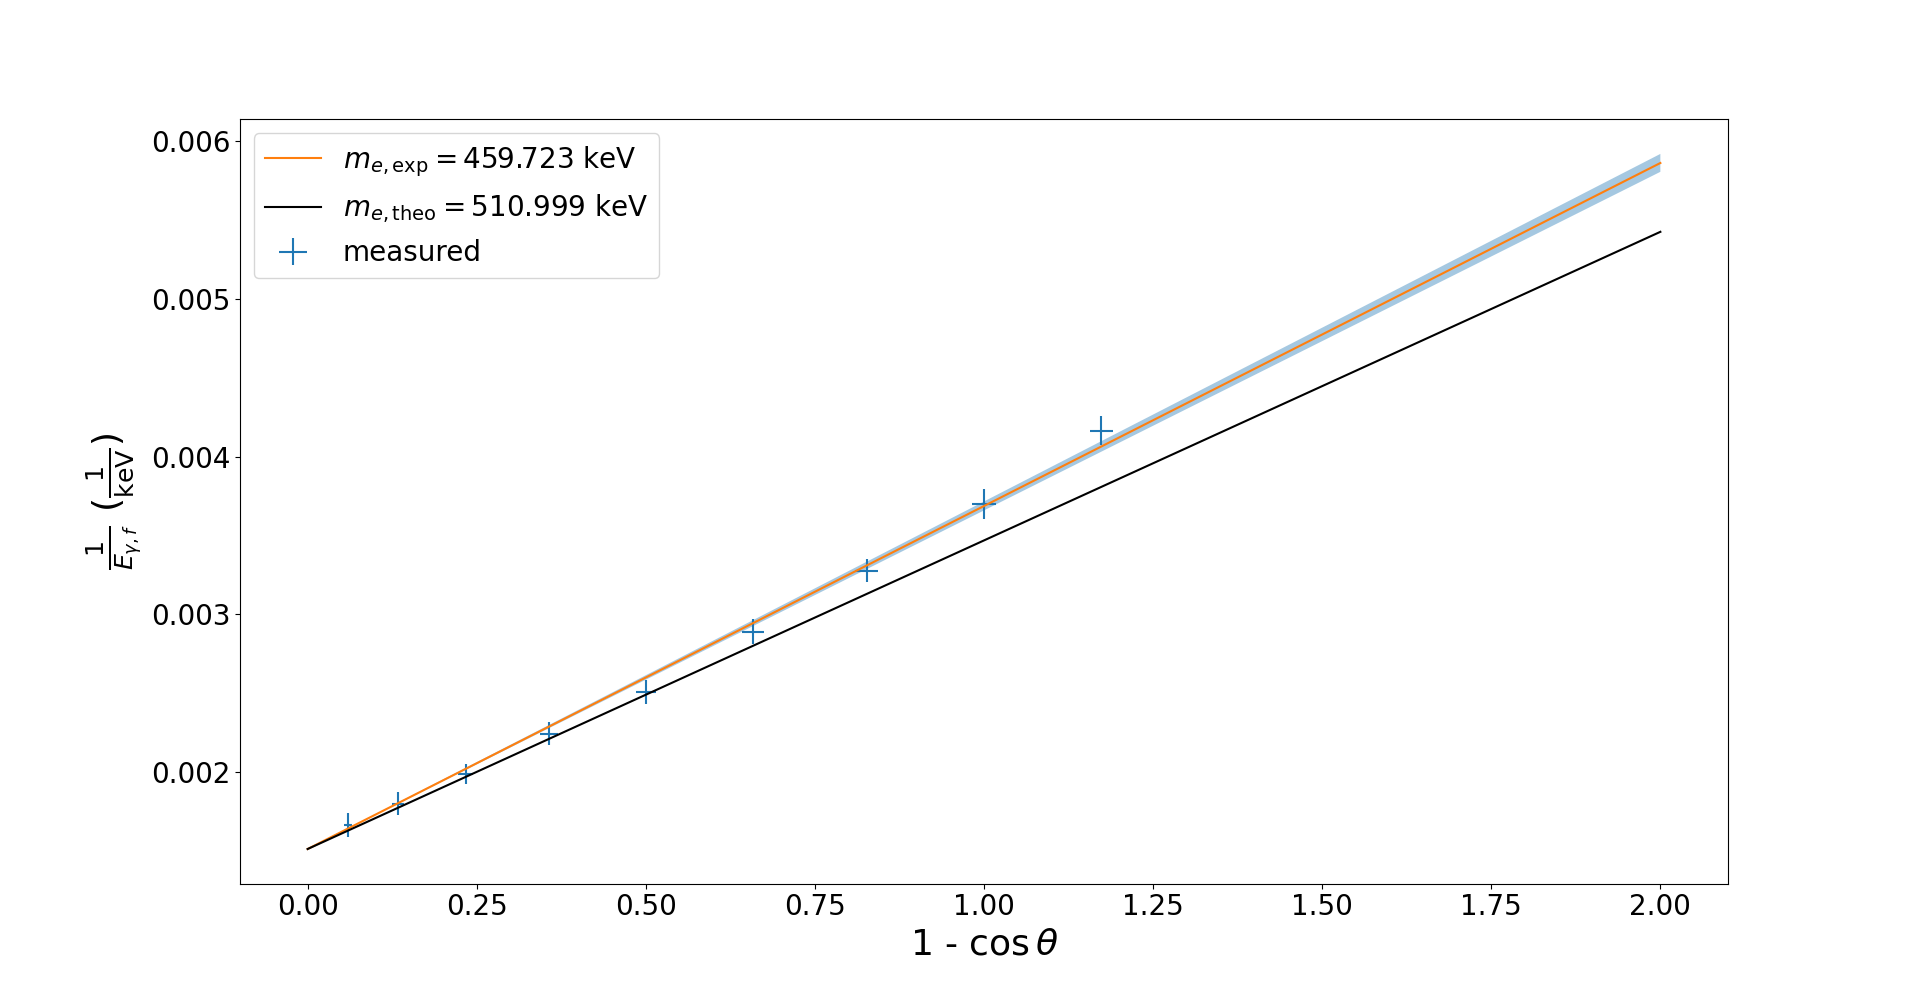
\includegraphics[width=1.0\textwidth]{./fig/energy-shift.png}
	\caption{Comparison of the calculated linear model with literature values.}
	\label{fig:energy-shift}
\end{figure}
